% LaTeX layout by Jonas Kahler, jonas@derkahler.de
% AutoTux Final Report
% Group Tux:
% Max Enelund, Jerker Ersare, Thorsteinn D. Jörundsson,
% Jonas Kahler, Dennis Karlberg Niklas le Comte, Marco Trifance, Ivo Vryashkov
% Chapter 5 - Software Architecture
\chapter{Software Architecture}
%% Low-level Board Software Architecture by Jerker
\section[Low-level Board Software Architecture]
{Low-level Board Software Architecture\textsuperscript{[JE]}}
The STM32 software consists of a main thread that reads sensor input values from
hardware components and forwards control data to the hardware 13.8 times per
second, and a serial thread that sends the sensor values to and reads control
data from the Odroid via the USB connection 20 times per second. The interaction
with hardware is explained further in the Hardware-Software Integration section
\textbf{[JONAS MAKE LINK]}.\\

\noindent
The hardware modules all have similar function names, to simplify their use. All
function names are prefixed with the source filename. We have taken care to
encapsulate the internal behaviour of all modules similar to the way common in
object oriented programming, so values are retrieved via \textit{getter}
functions. In our opinion, we managed to achieve a simple yet robust and easily
extensible architecture with modular aspects without wasting time
overgeneralising or over designing.
\newpage
\begin{figure}[ht]
  \centering
  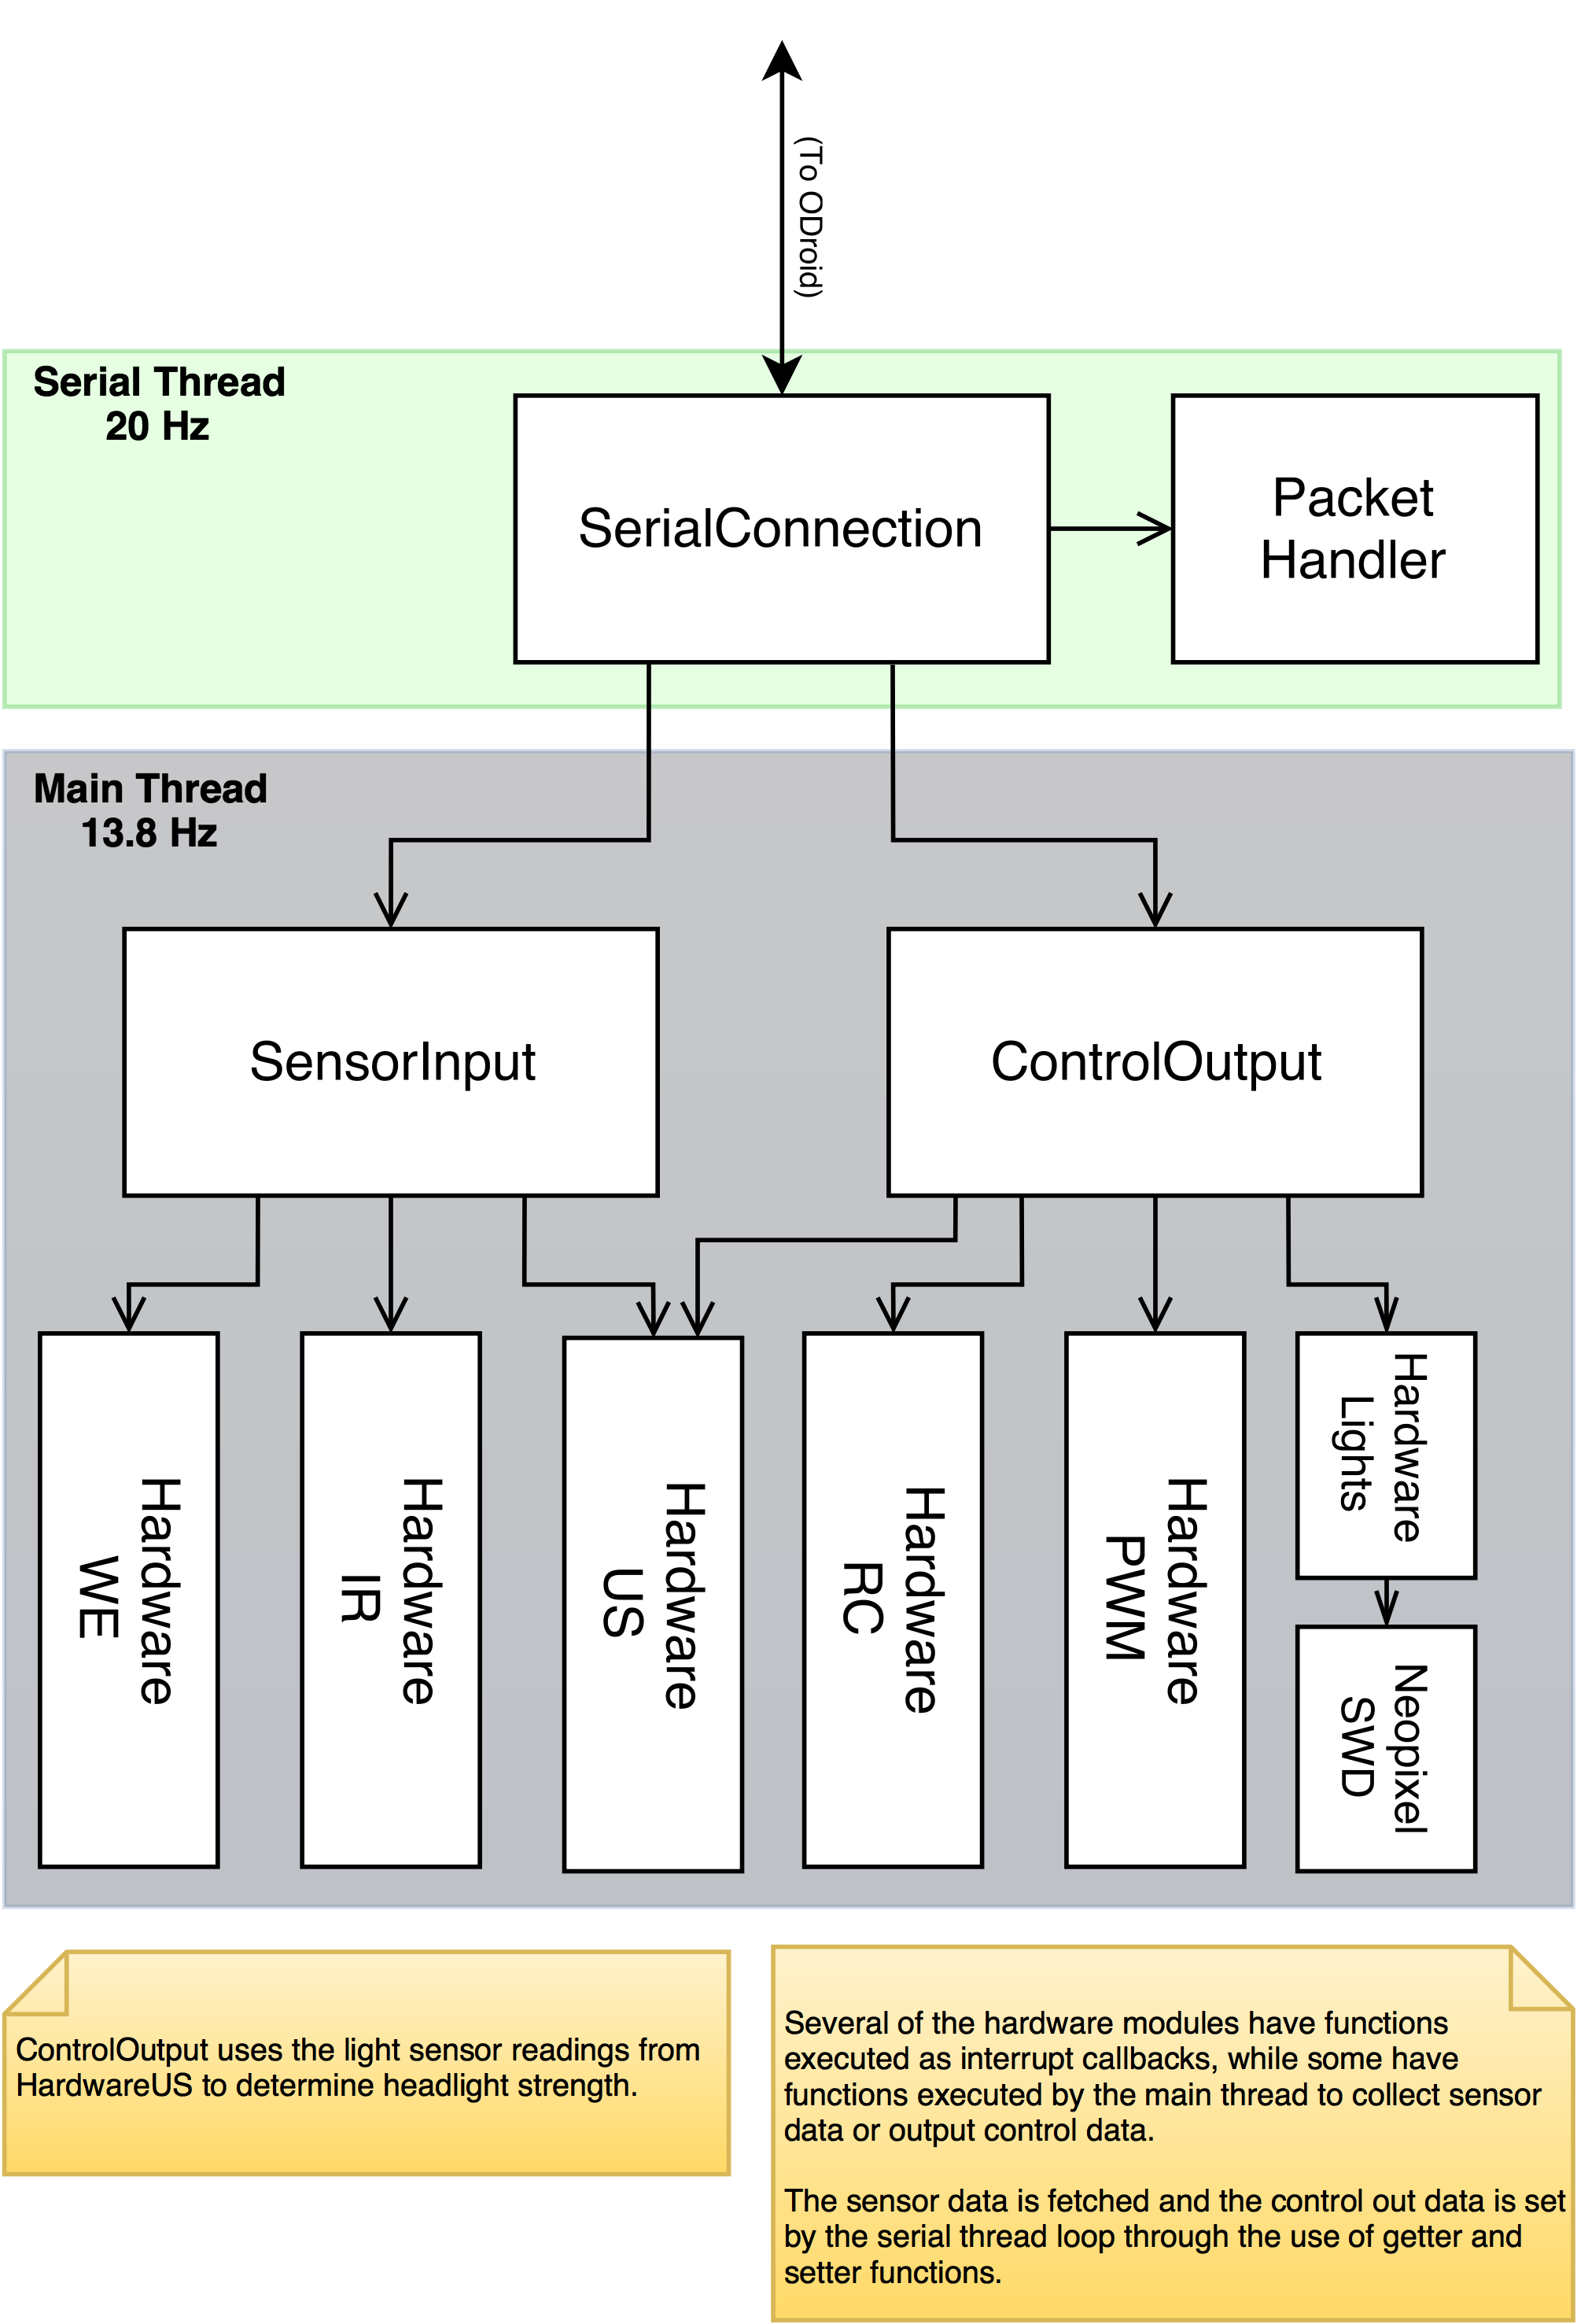
\includegraphics[height=15cm]{X-ThreadDiagram.png}
  \caption{STM32 Architecture}
  \label{xtdiagr}
\end{figure}

\newpage
%% High-level Board Archtiecture
\section{High-level Board Software Architecture}

%%% Overall Odroid Arch by Jonas & Dennis
\subsection[Overall Architecture]
{Overall Architecture\textsuperscript{[JK \& DK]}}
Initially we decided on running three different components: a proxy, a lane
follower and a decision maker component.\\
The proxy is responsible for exchanging the data with the low-level board and
putting the webcam image into the shared memory, the lane follower is
interpreting the webcam image and recommends steering angles and warns about
stoplines while the decision maker component finally takes and interprets this
data and decides on final steering wheel angle and speed. The decision maker
component also includes the logic for overtaking and parking.\\
We ended also up in having a fourth component running on the Odroid board: the
configuration tool. This tool’s purpose is to configure the lane-follower,
changing the main state, as well as looking at current sensor values.
\begin{figure}[ht]
  \centering
  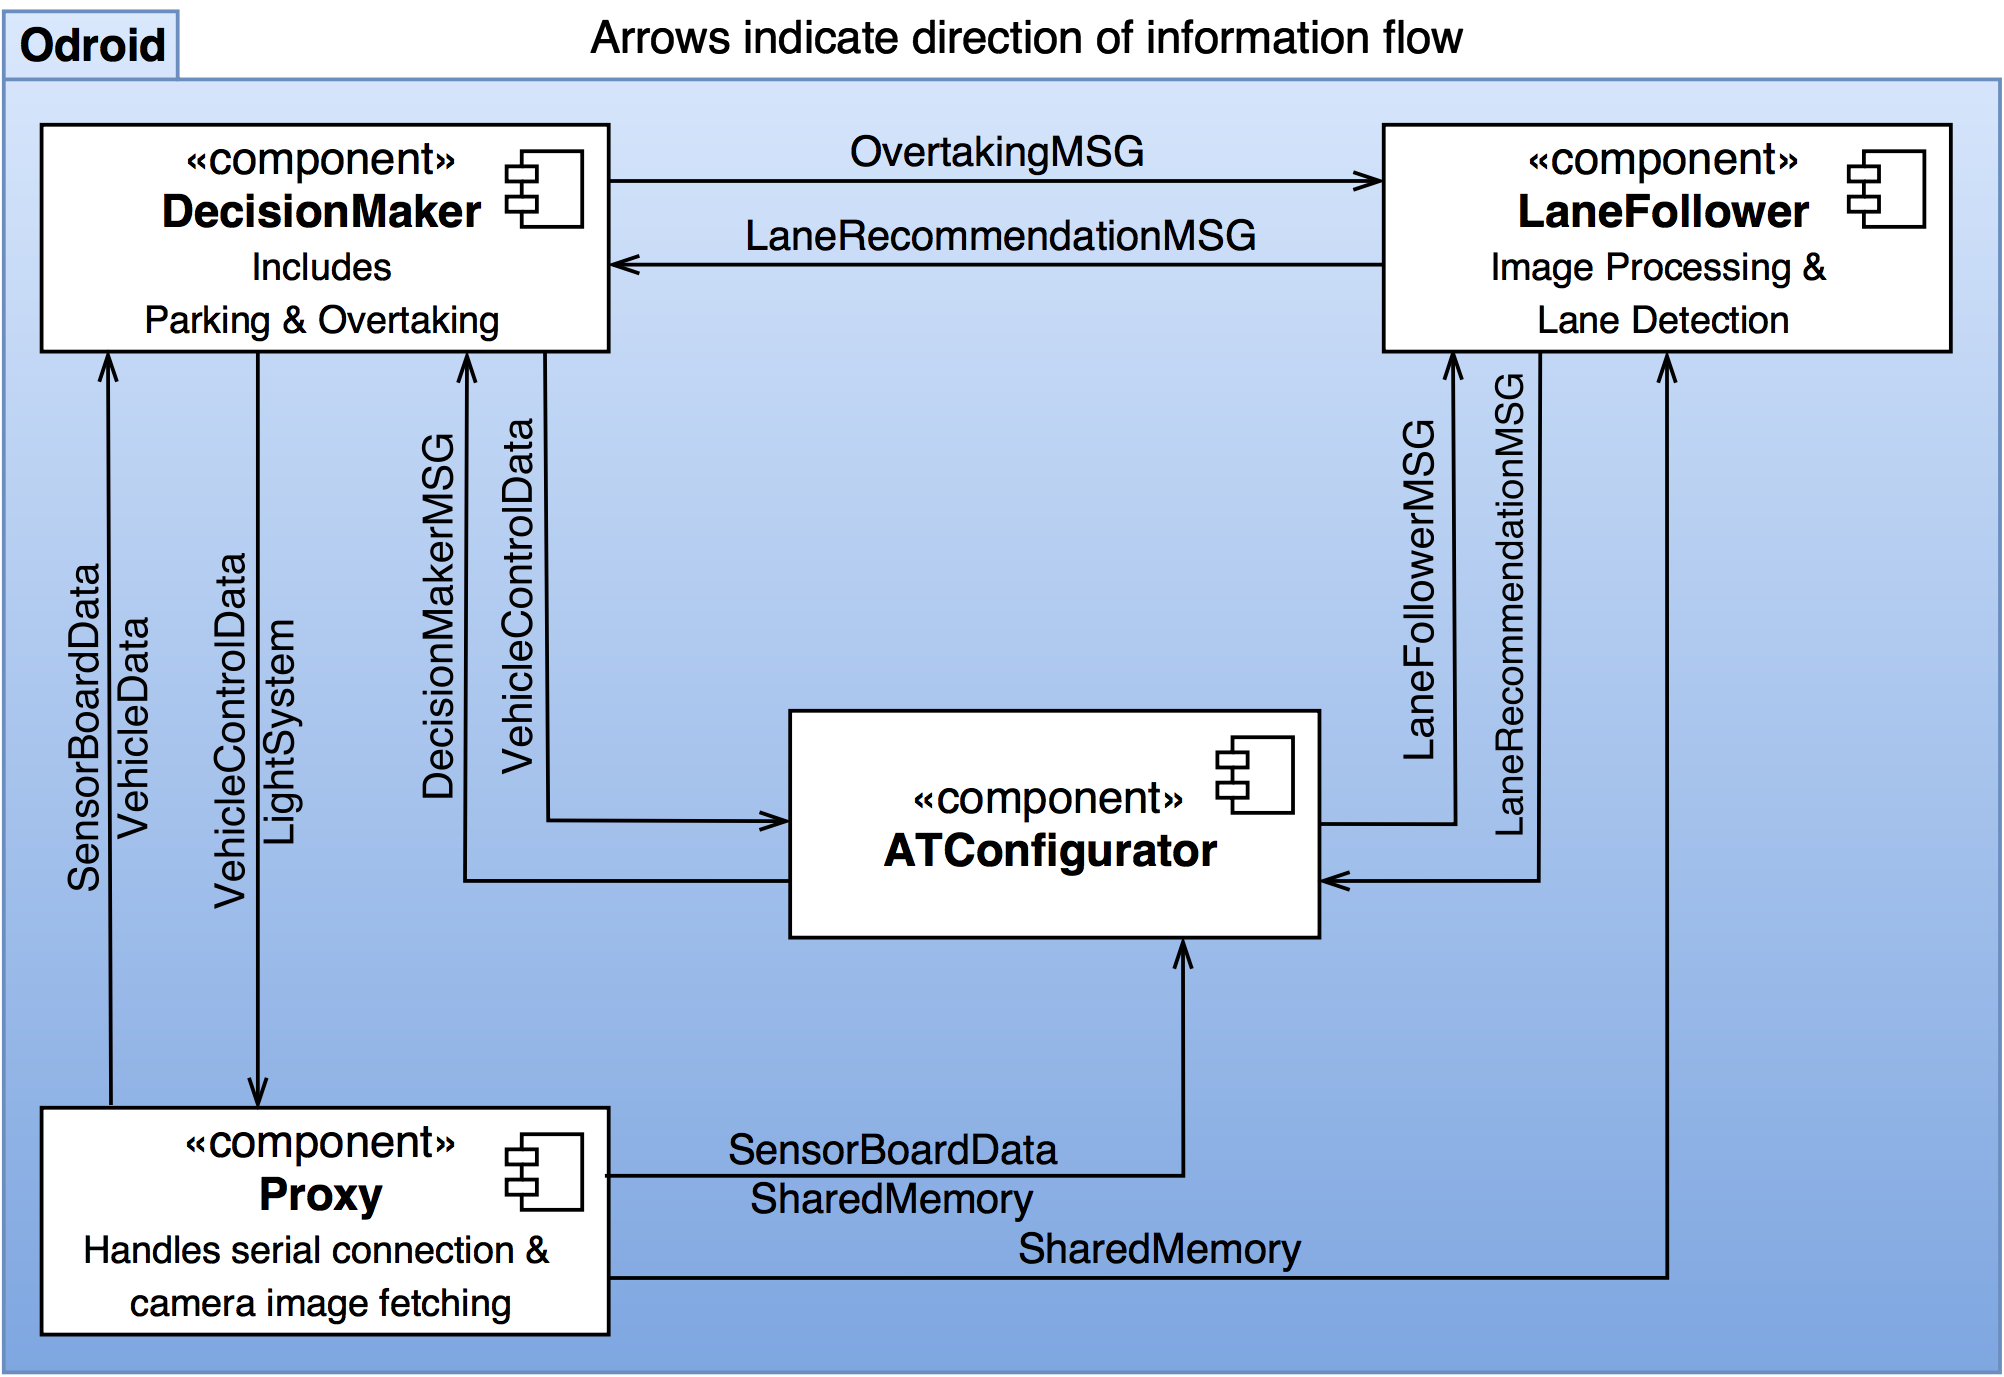
\includegraphics[width=1\textwidth]{X-ComponentDiagram.png}
  \caption{Odroid Architecture}
  \label{xcompdiagr}
\end{figure}
\newpage
\noindent
On the high-level board the data exchange works through the OD conference. All
components use the conference to share data between one another. When we started
out, the communication between the DecisionMaker and the LaneFollower was
one-directional. The LaneFollower simply used the shared image received from the
proxy component and and sent steering recommendations to the DecisionMaker.
However, due to our solution of the overtaking, we ended up having messages sent
both ways between the DecisionMaker and the LaneFollower.\\
The ATConfigurator component both sends and receives data from the DecisionMaker
and LaneFollower. As mentioned above, this component was used as a tool to
change and monitor data on the fly.\\
The data-flow between the Proxy and the DecisionMaker component is also
two-directional, the DecisionMaker retrieves sensor data from the Proxy and
sends vehicle control data back to the Proxy. Even though the data circulates a
lot to and from all components, it does not mean that they are dependent on one
another. The LaneFollower is only dependent on the Proxy component, as it can
not work without receiving an image. The DecisionMaker does not depend on any of
the other components. The same goes for the Proxy component.

%%% Communication Packets by Ivo
\subsection[Communication Packets]{Communication Packets\textsuperscript{[IV]}}
We used Netstring for the structure of our data packets. This allowed us to keep
our packets small and compact. The sensor-board data packet has the following
outline:
\begin{center}
\textit{12 : us1 us2 ir1 ir2 ir3 speed dis1 dis2 dis3 dis4 light checksum ,}
\end{center}
In the above, \textit{12} is the number of elements in the packet, \textit{:}
is the start delimiter and \textit{,} is the end delimiter. The length header
and the delimiters are written in ascii characters. Each element in the packet
body is an unsigned char. The values for the different sensors, i.e. ultrasonic
and infrared, are holding integer values 0-255. The speed is in centimeters per
second. The dis1-4 represent the distance travelled as a four-byte integer.
Light represents the light sensor reading of the surrounding brightness.

\newpage
\noindent
The vehicle-control data packet is as follows:
\begin{center}
\textit{4 : speed angle lights checksum ,}
\end{center}
The outline of the packet follows the same convention as the sensor-board data.
For the speed, we used an enum for the different types, i.e. 0 is backward, 1 is
stopped, 2 is forward and 3 is cruise speed. The angle values are converted from
radians to degrees (centered around 90 degrees instead of 0 to stay in the
unsigned range). The lights are controlled by setting the bits for the different
states - bit 0 (rightmost bit) for brake, bit 1 for reverse, bit 2 for flashing
left and bit 3 for flashing right.

%%% Configuration Tool by Jonas
\subsection[Configuration Tool]{Configuration Tool\textsuperscript{[JK]}}
The configuration tool contains of two separate threads running:\\
The first thread is the main thread of the application. The
\textit{TimeTriggeredConferenceClientModule} provided by OpenDaVINCI runs in
that very thread.\\
The second thread is the TUIs main loop which is basically a while loop running
at roughly 40Hz. This loop refreshes all ncurses windows in a rate which feels
instant to the user as well as reading the input commands from the keyboard
(which is non blocking because of the usage of ncurses no-delay mode.\\

\noindent
As mentioned in [Implementation Details Section link], a Singleton class is used
to exchange data between the \textit{TimeTriggeredConferenceClientModule} and
the TUI. The decision for a Singleton was made to avoid passing around an object
to every single of the using classes.\\
It is certainly not an optimal solution, but in our opinion ``good enough''.\\

\noindent
Because \textit{ncurses} is a library written in C, some decisions were made to
make it fit more into our object oriented code written in C++:\\
Each ncurses window got wrapped into a separate object, having member functions
necessary for effecting this window. Eg: each ncurses window object draws itself
with the help of the \textit{void refresh(void);} member function.
